\documentclass[fleqn,varvw,preprintnumbers,citeautoscript]{memo}

\usepackage[utf8]{inputenc}
\usepackage[T1]{fontenc}

\graphicspath{{../../fig/}}
\usepackage[caption=false]{subfig}
\usepackage{enumerate}


\newcommand\vlong{V_\text{long}}

\begin{document}

\title{Memo 3: schema circuitale completo}

\author{Francesco Polleri}
\email{s5025011@studenti.unige.it}
\author{Mattia Sotgia}
\email{s4942225@studenti.unige.it}

\collaboration{Gruppo A1}
\affiliation{Dipartimento di Fisica, Università degli Studi di Genova, I-16146 Genova, Italia}

\author{Lorenzo Lucentini}
\author{Michele Giorgi}
\collaboration{Gruppo C6}
\affiliation{Dipartimento di Fisica, Università degli Studi di Genova, I-16146 Genova, Italia}

\revised{\today}
\preprint{MEMO/3 (\today)}

\begin{abstract}

\end{abstract}
\maketitle

\begin{turnpage}
    \begin{figure*}[p]
        \centering
        % 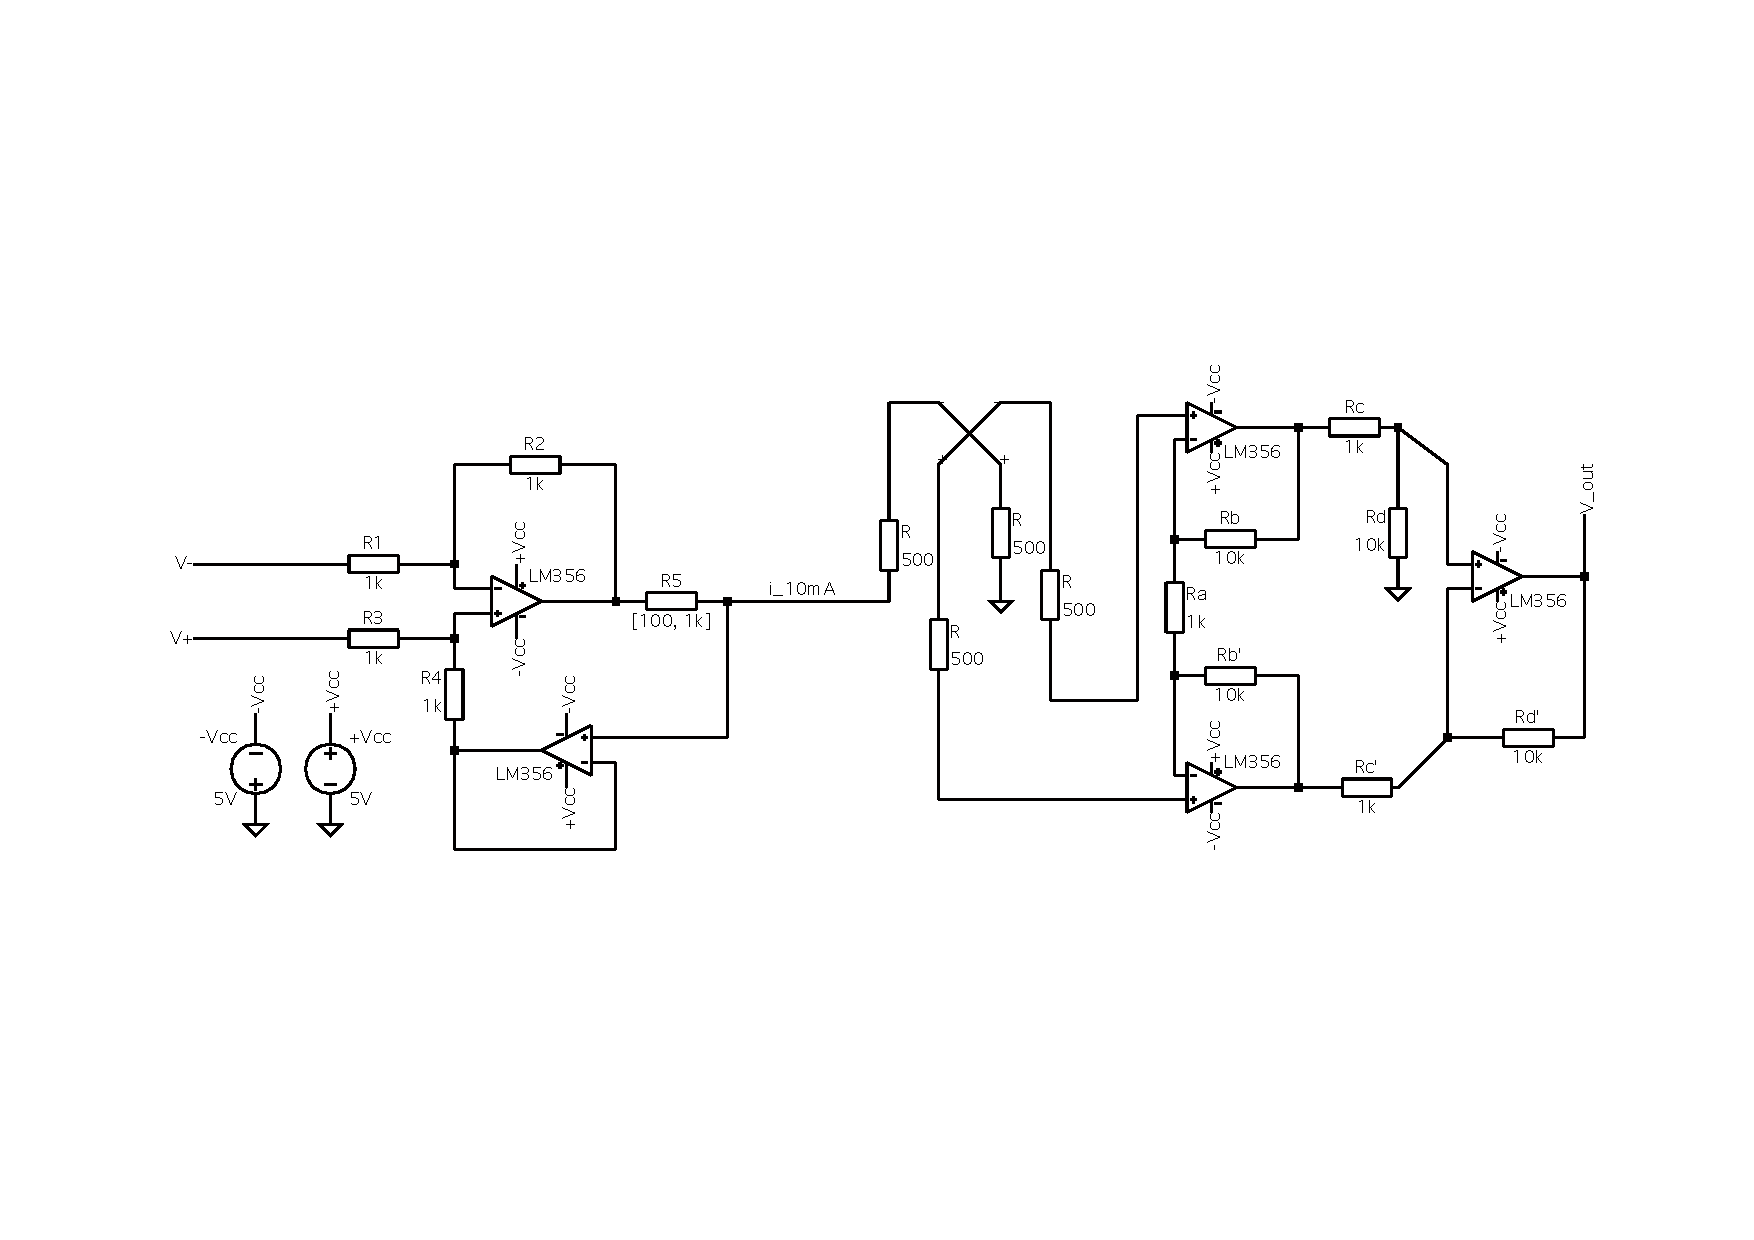
\includegraphics[width=\linewidth,trim={2cm 6.5cm 2cm 6cm},clip]{memo2_full_circuit.pdf}
        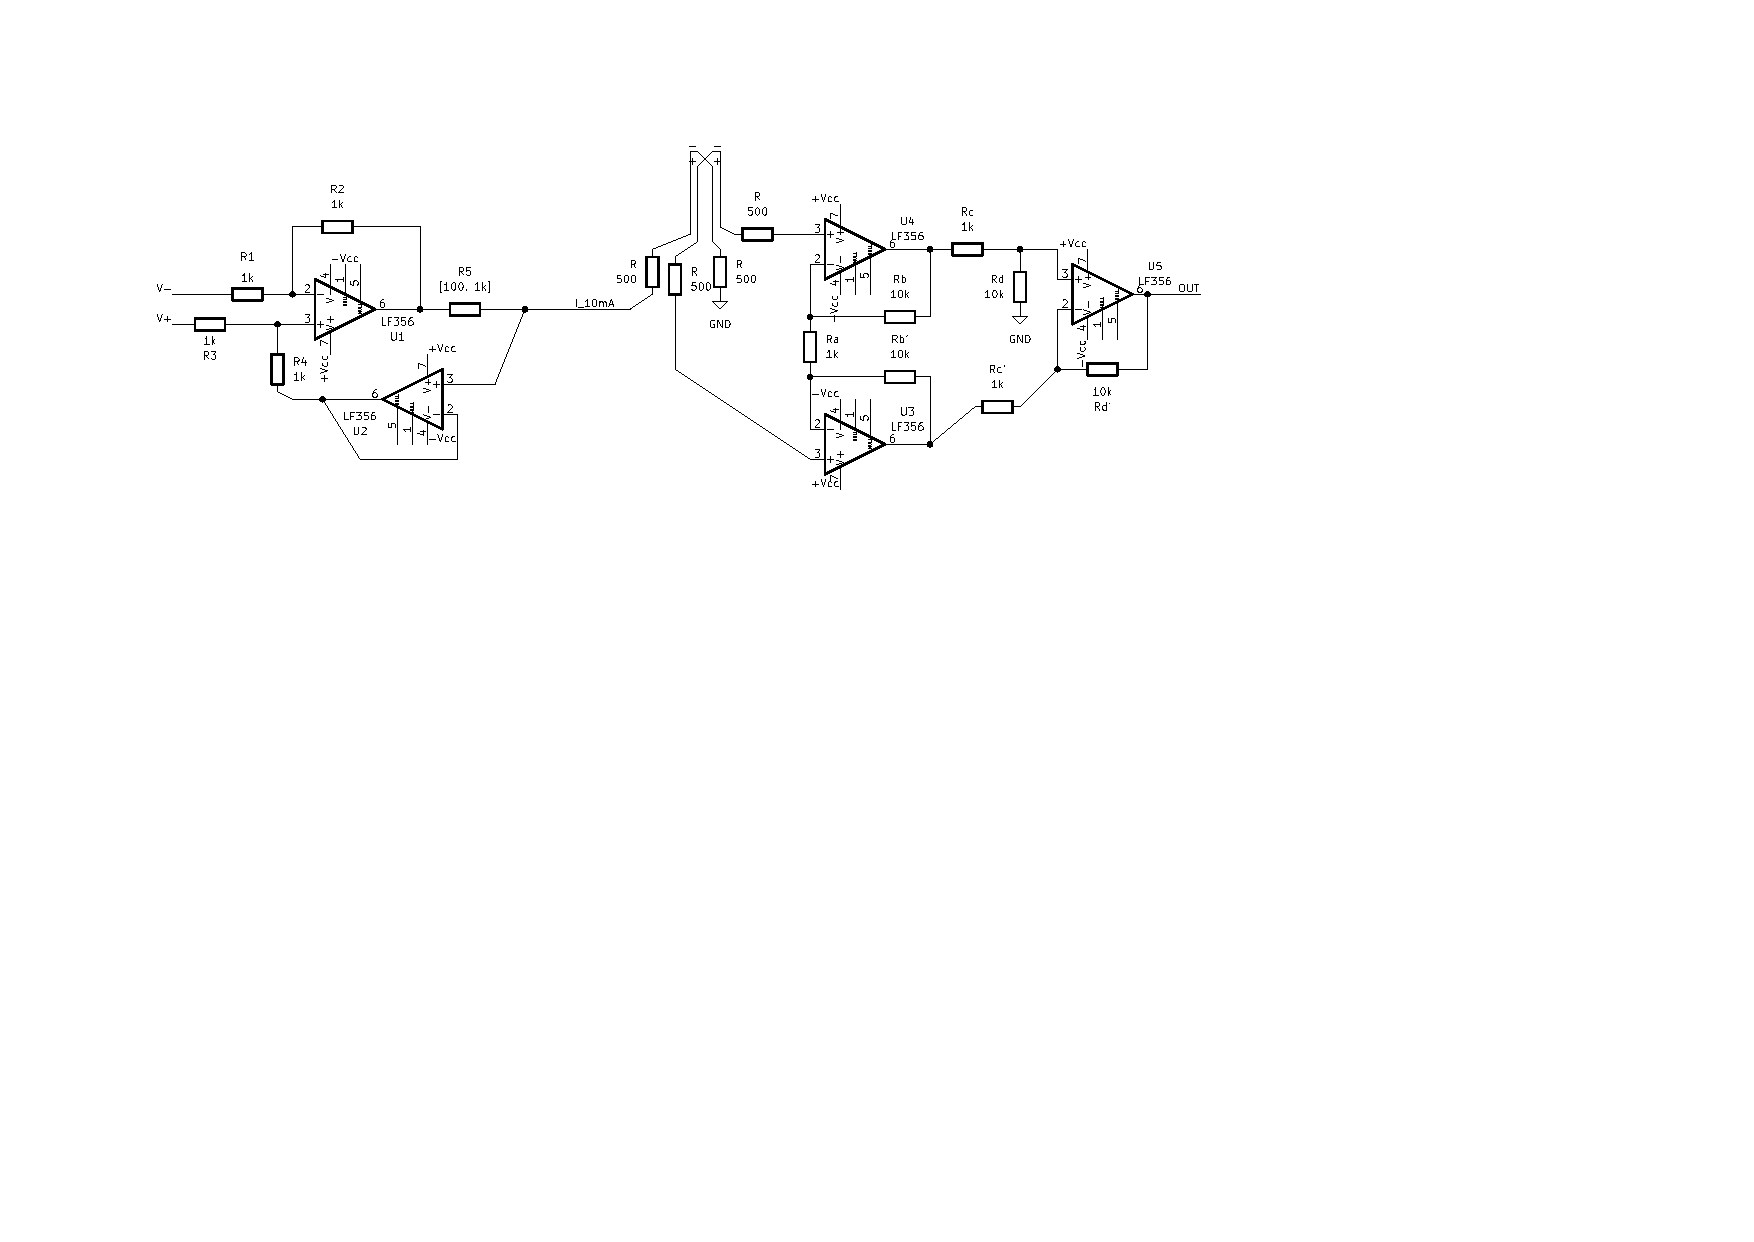
\includegraphics[width=\linewidth,trim={2.5cm 3.5cm 2cm 2cm},clip]{SCHEMA_full1.pdf}
        \caption{Circuito completo delle tre componenti principali (da sinistra a destra sono inseriti il generatore di corrente, la sonda e l'amplificatore differenziale per strumentazione). In basso a destra troviamo la scheda Arduino MEGA 2560 mappata sui pin utilizzati per il setup sperimentale. }\label{fig:circuit_memo2}
    \end{figure*}
\end{turnpage}

\end{document}